\section{Einführung}
Eine reale Spannungsquelle wird durch das Modell des Innenwiderstandes beschrieben. Dabei wird gerechnet, als wäre ein Innenwiderstand $R_i$ in Reihe mit der eigentlichen Spannungsquelle mit Leerlaufspannung $U_0$ geschaltet. Es ergibt sich bei Belastung durch einen Außenwiderstand $R_a$ (Strom $I$):
\begin{equation}
  U_0=R_i\cdot I+R_a\cdot I
  \label{eq:innenwiderstand}
\end{equation}
Die tatsächlich gemessene Spannung an der Quelle weicht von der Leerlaufspannung ab und heißt Klemmspannung $U_{\text{Kl}}$:
\begin{equation}
  U_{\text{Kl}}=U_0-R_i\cdot I=R_a\cdot I
  \label{eq:klemmspannung}
\end{equation}
Beim Kurzschluss für $R_a=0$ fließt der endliche Strom
\begin{equation}
  I_{\text{Ks}}=U_0/R_i.
  \label{eq:kurzschluss}
\end{equation}
Die an den Verbraucher abgegebene Leistung beträgt
\begin{equation}
  P=U_0^2 \frac{R_a}{(R_a+R_i)^2}.
  \label{eq:leistung}
\end{equation}
Wir leiten die Bedingung für maximale Leistungsabgabe her:
\begin{align}
  &\frac{\mathrm{d}P}{\mathrm{d}R_a}=\frac{U_0^2}{(R_a-R_i)^2}-2\cdot \frac{R_a U_0^2}{(R_a+R_i)^3}=0 \\
  &\implies (R_a+R_i)=2R_a \implies R_a=R_i
  \label{eq:maxleistung}
\end{align}

\section{Versuche}
\subsection{Aufgabe 1}
Ziel dieses Versuches ist die Bestimmung von Leerlaufspannung $U_0$ und Innenwiderstand $R_i$ von
\begin{enumerate}
  \item einer einzelnen Akkumulatorzelle
  \item drei Zellen parallel
  \item drei Zellen in Reihe.
\end{enumerate}
Dazu wird ein Stöpselwiderstand $R_a$ in Reihe und ein Spannungsmessgerät zur Messung der Klemmspannung $U_{\text{Kl}}$ parallel zu den Zellen geschaltet. Der Stöpselwiderstand fungiert als Lastwiderstand, über den der Strom $I$ reguliert werden kann. Es werden jeweils 13 Spannungswerte nach Einstellen verschiedener Widerstände $R_a$ abgenommen. Darunter sind auch Werte für den Kurzschlussfall ($R_a$=0) und für nicht geschlossenen Stromkreis ($R_a=\infty$).
\begin{table}[H]
  \centering
  \begin{tabular}{c c c} \toprule
    $R_a$ [\SI{\pm1}{\ohm}] & $U_{\text{Kl}}$ [\SI{\pm .015}{V}] & $I=U_{\text{Kl}}/R_a$ [\SI{\pm .5}{mA}] \\ \midrule
    $\infty$ & \num{1.338} & - \\
    0 & \num{0.021} & - \\
    5 & \num{0.303} & \num{60.6} \\
    10 & \num{.483} & \num{48.3} \\
    20 & \num{.717} & \num{35.8} \\
    30 & \num{.840} & \num{28.0} \\
    40 & \num{.930} & \num{23.3} \\
    50 & \num{.987} & \num{19.7} \\
    60 & \num{1.035} & \num{17.3} \\
    70 & \num{1.071} & \num{15.3} \\
    80 & \num{1.095} & \num{13.7} \\
    90 & \num{1.113} & \num{12.4} \\
    100 & \num{1.140} & \num{11.4} \\ \bottomrule
  \end{tabular}
  \caption{Messergebnis für eine Zelle}
  \label{tab:einezelle}
\end{table}

\begin{table}[H]
  \centering
  \begin{tabular}{c c c} \toprule
    $R_a$ [\SI{\pm 1}{\ohm}] & $U_{\text{Kl}}$ [\SI{\pm .05}{V}] & $I=U_{\text{Kl}}/R_a$ [\SI{\pm 1.2}{mA}] \\ \midrule
    $\infty$ & \num{4.00} & - \\
    0 & \num{0.10} & - \\
    5 & \num{0.40} & \num{80} \\
    10 & \num{.70} & \num{70} \\
    20 & \num{1.15} & \num{57.5} \\
    30 & \num{1.48} & \num{49.3} \\
    40 & \num{1.73} & \num{43.3} \\
    50 & \num{1.98} & \num{39.6} \\
    60 & \num{2.12} & \num{35.3} \\
    70 & \num{2.30} & \num{32.9} \\
    80 & \num{2.40} & \num{30.0} \\
    90 & \num{2.52} & \num{28.0} \\
    100 & \num{2.61} & \num{26.1} \\ \bottomrule
  \end{tabular}
  \caption{Messergebnis für drei Zellen parallel}
  \label{tab:einezelle}
\end{table}

\begin{table}[H]
  \centering
  \begin{tabular}{c c c} \toprule
    $R_a$ [\SI{\pm1}{\ohm}] & $U_{\text{Kl}}$ [\SI{\pm .015}{V}] & $I=U_{\text{Kl}}/R_a$ [\SI{\pm .5}{mA}] \\ \midrule
    $\infty$ & \num{1.323} & - \\
    0 & \num{0.030} & - \\
    5 & \num{0.327} & \num{65.4} \\
    10 & \num{.495} & \num{49.5} \\
    20 & \num{.717} & \num{35.9} \\
    30 & \num{.843} & \num{28.1} \\
    40 & \num{.930} & \num{23.3} \\
    50 & \num{.990} & \num{19.8} \\
    60 & \num{1.023} & \num{17.1} \\
    70 & \num{1.068} & \num{15.3} \\
    80 & \num{1.095} & \num{13.7} \\
    90 & \num{1.113} & \num{12.4} \\
    100 & \num{1.137} & \num{11.4} \\ \bottomrule
  \end{tabular}
  \caption{Messergebnis für drei Zellen in Reihe}
  \label{tab:einezelle}
\end{table}
Wir beobachten bei allen drei Messungen eine Zunahme der Klemmspannung $U_{\text{Kl}}$ und Abnahme des Stromes $I$ bei höherem Lastwiderstand $R_a$. Die Werte für eine Zelle entsprechen bis auf geringe Abweichungen den Werten für drei Zellen in Reihe. Die größte Abweichung tritt für $R_a=\SI{5}{\ohm}$ auf und beträgt $\Delta U_0=(\SI{0.327}{V}-\SI{0.303}{V})/(\SI{0.303}{V})\approx \SI{8}{\percent}$.

\subsection{Aufgabe 4}
Da es keine weiteren Angaben zur Frequenz der Wechselspannung gab, wurde von den normalen 50 Hz ausgegangen.
\begin{figure}[H] 
  \centering
	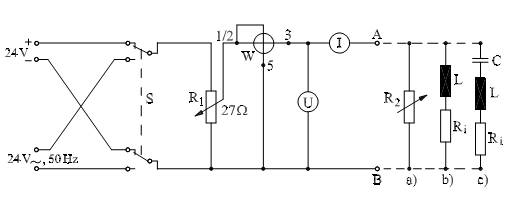
\includegraphics[width=0.7\textwidth]{Schaltplan.png}
	\caption{Schaltplan für die Aufgaben 4-8 \footcite{anleitung-ws2014}}
  \label{fig:kreisel1}
\end{figure}
In dem Aufbau wird kein Verbraucher angeschlossen um die Verlustleistung des Voltmeters zu bestimmen. Diese beträgt bei maximaler Spannung, $U_{Gleich}=27V$ oder $U_{Wechsel}=25,5V$, $P_{verlust}=1W$ und nimmt bei sinkenden Spannungen weiter ab.
\subsection{Aufgabe 5}
An den Punkten A und B wird ein ohmscher Widerstand angeschlossen, für den bei Wechsel- und Gleichspannung die möglichen Messwerte bestimmt werden.
\begin{table}[H]
  \centering
  \begin{tabular}{c | c | c | c}
    Spannungsart & Spannung U [V] $\pm0,25$ & Stromstärke I [A] $\pm 0,05$ & Leistung P [W] $\pm0,5$\\ \hline
     & 24 & 1,00 & 23,7\\
     & 20 & 0,85 & 17,0\\
     Wechselspannung & 15 & 0,68 & 9,8\\
     & 10 & 0,43 & 4,0\\
     & 5 & 0,20 & 1,0\\ \hline
     & 25 & 1,00 & 24,5\\
     & 20 & 0,82 & 16,0\\
     Gleichspannung & 15 & 0,63 & 9,0\\
     & 10 & 0,42 & 3,9\\
     & 5 & 0,20 & 0,6
  \end{tabular}
  \caption{Messwerte des ohmschen Widerstands}
  \label{tab:messungohm}
\end{table}
\begin{figure}[H]
  \centering
  \begin{tikzpicture}
    \begin{axis}[
      width=15 cm,
      height=9 cm,
      xmin=0, xmax=30,
      ymin=0, ymax=1.2,
      xlabel={Angelenkte Spannung U [V]},
      ylabel={Gemessene Stromstärke I [A]},
      legend entries={Gleichspannung, Wechselspannung, Linearer Fit beider Spannungen},
      legend pos=north west,
      domain=0.1:28,
    ]
      \addplot plot [only marks,mark=x,thick,error bars/.cd, x dir=both, x fixed=0.25, y dir=both, y fixed=0.05]  file {GleichR.txt};
      \addplot plot [only marks,mark=o,thick,error bars/.cd, x dir=both, x fixed=0.25, y dir=both, y fixed=0.05]  file {WechselR.txt};
      \addplot[mark=none] {0.04*x+0.014};
    \end{axis}
  \end{tikzpicture}
  \caption{Versuch mit ohmschen Widerstand (Spannung gegen Stromstärke)}
  \label{fig:UIOhmscher}
\end{figure}
In dem Diagramm wurde nur der Fit für Gleichspannung eingetragen, da sich dieser fast mit dem von der Wechselspannung deckt und so eine größere Übersichtlichkeit erreicht wurde.

Aufgrund des anscheinend sehr linearen Verlaufs der Messwerte für beide Spannungsarten und in Deckung mit der zu erwarteten Formel \ref{eq:Rohm} wurde mit \emph{gnuplot} nach dem \emph{least-squares}-Verfahren die Werte der beiden Spannungsarten gegen die Funktion $f(x)=m\cdot x+b$ gefittet. Ausgabe:
\begin{table}[H]
  \centering
  \begin{tabular}{c | c | c | c}
    Spannungsart & Variabel m & Variabel b & Varians der Residuals\\ \hline
    Gleichspannung & 0,04 & 0,014 & 0,00024\\
    Wechselspannung & 0,0422 & 0,007 & 0,00077
  \end{tabular}
  \caption{Linearer Fit zu Abbildung \ref{fig:UIOhmscher}}
  \label{tab:fitUIOhmscher}
\end{table}
\begin{figure}[H]
  \centering
  \begin{tikzpicture}
    \begin{axis}[
      width=15 cm,
      height=9 cm,
      xmin=0, xmax=25,
      ymin=0, ymax=30,
      xlabel={Gemessene Leistung P [W]},
      ylabel={Produkt der Stromstärke I und der Spannung U [W]},
      legend entries={Gleichspannung, Wechselspannung, Linearer Fit beider Spannungen},
      legend pos=north west,
      domain=0.1:28,
    ]
      \addplot plot [only marks,mark=x,thick,error bars/.cd, x dir=both, x fixed=0.5, y dir=both, y fixed=0.5]  file {GleichR4.txt};
      \addplot plot [only marks,mark=o,thick,error bars/.cd, x dir=both, x fixed=0.5, y dir=both, y fixed=0.5]  file {WechselR2.txt};
      \addplot[mark=none] {1.005*x+0.352};
    \end{axis}
  \end{tikzpicture}
  \caption{Versuch mit ohmschen Widerstand (Leistung gegen Produkt aus Spannung und Stromstärke)}
  \label{fig:PUIOhmscher}
\end{figure}
In dem Diagramm wurde nur der Fit für Gleichspannung eingetragen, da sich dieser fast mit dem von der Wechselspannung deckt und so eine größere Übersichtlichkeit erreicht wurde. Der Fehler des Produktes von Stromstärke und Spannung wurde nach der Gaußschen Fehlerfortpflanzung bestimmt.

Aufgrund des anscheinend linearen Verlaufs der Messwerte für beide Spannungsarten und in Deckung mit der zu erwarteten Formel \ref{eq:leistung} wurde mit \emph{gnuplot} nach dem \emph{least-squares}-Verfahren die Werte der beiden Spannungsarten gegen die Funktion $f(x)=m\cdot x+b$ gefittet. Ausgabe:
\begin{table}[H]
  \centering
  \begin{tabular}{c | c | c | c}
    Spannungsart & Variabel m & Variabel b & Varians der Residuals\\ \hline
    Gleichspannung & 1,005 & 0,352 & 0,004\\
    Wechselspannung & 1,003 & 0,164 & 0,45
  \end{tabular}
  \caption{Linearer Fit zu Abbildung \ref{fig:PUIOhmscher}}
  \label{tab:fitPUIOhmscher}
\end{table}
\subsection{Aufgabe 6}
In diesem Versuchsteil wird eine Spule an den Punkten A und B angeschlossen (Aufbau b), und für Wechselspannung die Messwerte bestimmt.
\begin{table}[H]
  \centering
  \begin{tabular}{c | c | c}
    Spannung U [V] $\pm0,25$ & Stromstärke I [A] $\pm 0,05$ & Leistung P [W] $\pm0,5$\\ \hline
    25 & 0,85 & 16,2\\
    20 & 0,67 & 10,8\\
	15 & 0,50 & 6,0\\
    10 & 0,33 & 2,5\\
    5 & 0,20 & 1,0\\ 
  \end{tabular}
  \caption{Messwerte der Spule bei Wechselspannung}
  \label{tab:messungspulewechsel}
\end{table}
\begin{figure}[H]
  \centering
  \begin{tikzpicture}
    \begin{axis}[
      width=15 cm,
      height=9 cm,
      xmin=0, xmax=30,
      ymin=0, ymax=1.2,
      xlabel={Angelenkte Spannung U [V]},
      ylabel={Gemessene Stromstärke I [A]},
      legend entries={Wechselspannung, Linearer Fit},
      legend pos=north west,
      domain=0.1:28,
    ]
      \addplot plot [only marks,mark=x,thick,error bars/.cd, x dir=both, x fixed=0.25, y dir=both, y fixed=0.05]  file {WechselL.txt};
      
      \addplot[mark=none] {0.034*x-0.0096};
    \end{axis}
  \end{tikzpicture}
  \caption{Versuch mit Spule (Spannung gegen Stromstärke)}
  \label{fig:UISpule}
\end{figure}
\begin{table}[H]
  \centering
  \begin{tabular}{c | c | c | c}
    Spannungsart & Variabel m & Variabel b & Varians der Residuals\\ \hline
    Wechselspannung & 0,034 & -0,0096 & $2,54\cdot10^{-5}$
  \end{tabular}
  \caption{Linearer Fit zu Abbildung \ref{fig:UISpule}}
  \label{tab:fitUISpule}
\end{table}
\begin{figure}[H]
  \centering
  \begin{tikzpicture}
    \begin{axis}[
      width=15 cm,
      height=9 cm,
      xmin=0, xmax=20,
      ymin=0, ymax=25,
      xlabel={Leistung P [W]},
      ylabel={Produkt der Stromstärke I und der Spannung U [W]},
      legend entries={Wechselspannung, Linearer Fit},
      legend pos=north west,
      domain=0.1:28,
    ]
      \addplot plot [only marks,mark=x,thick,error bars/.cd, x dir=both, x fixed=0.5, y dir=both, y fixed=0.5]  file {WechselL2.txt};
      
      \addplot[mark=none] {1.301*x-0.171};
    \end{axis}
  \end{tikzpicture}
  \caption{Versuch mit Spule (Leistung gegen Produkt aus Spannung und Stromstärke)}
  \label{fig:PUISpule}
\end{figure}
Der Fehler des Produktes von Stromstärke und Spannung wurde nach der Gaußschen Fehlerfortpflanzung bestimmt.
\begin{table}[H]
  \centering
  \begin{tabular}{c | c | c | c}
    Spannungsart & Variabel m & Variabel b & Varians der Residuals\\ \hline
    Wechselspannung & 1,301 & -0,171 & 0,14
  \end{tabular}
  \caption{Linearer Fit zu Abbildung \ref{fig:PUISpule}}
  \label{tab:fitPUISpule}
\end{table}
Aus dem Fit \ref{tab:fitPUISpule} ergibt sich, wenn man den $b$ Achsenabschnitt, der aus Messungenauigkeiten folgt, vernachlässigt,
\begin{equation}
U\cdot I=1,301\cdot P.
\end{equation}
Wenn man dies nun in \ref{eq:phase} einsetzt und nach dem Phasenwinkel $\varphi$ auflöst, erhält man
\begin{equation}
\varphi = \pm arccos(\frac{1}{1,301}) = \pm 39,77^\circ.
\end{equation}
Da es sich um eine Schaltung bestehend aus nur einer Spule handelt, kann man allgemein sagen, dass die Stromstärke der Spannung folgt, woraus folgt, dass gilt
\begin{equation}
\varphi = 39,77^\circ.
\end{equation}

Aus dem Fit \ref{tab:fitUISpule} ergibt sich unter der Vernachlässigung von b
\begin{equation}
I=0,034\Omega^{-1}\cdot U.
\end{equation}
Wenn man dies nun in die Formel \ref{eq:wirkohm} einsetzt erhält man
\begin{equation}
R_W=\frac{U}{I}cos(\varphi)=\frac{U}{0,034\Omega^{-1}\cdot U}cos(\varphi)=\frac{1}{0,034\Omega^{-1}}cos(\varphi)= \frac{500}{17}cos(\varphi)\Omega \approx 22,61 \Omega
\end{equation}
\subsection{Aufgabe 7}
\begin{table}[H]
  \centering
  \begin{tabular}{c | c }
    Spannung U [V] $\pm0,25$ & Stromstärke I [A] $\pm 0,05$ \\ \hline
    24,5 & 1,0 \\
    19,0 & 0,8\\
	14,0 & 0,6 \\
    9,1 & 0,4 \\
    5,0 & 0,2 \\ 
  \end{tabular}
  \caption{Messwerte der Spule bei Wechselspannung}
  \label{tab:messungspulegleich}
\end{table}
\begin{figure}[H]
  \centering
  \begin{tikzpicture}
    \begin{axis}[
      width=15 cm,
      height=9 cm,
      xmin=0, xmax=30,
      ymin=0, ymax=1.2,
      xlabel={Angelenkte Spannung U [V]},
      ylabel={Gemessene Stromstärke I [A]},
      legend entries={Gleichspannung, Linearer Fit},
      legend pos=north west,
      domain=0.1:28,
    ]
      \addplot plot [only marks,mark=x,thick,error bars/.cd, x dir=both, x fixed=0.25, y dir=both, y fixed=0.05]  file {GleichL.txt};
      
      \addplot[mark=none] {0.041*x+0.016};
    \end{axis}
  \end{tikzpicture}
  \caption{Versuch mit Spule}
  \label{fig:UIGleichSpule}
\end{figure}
\begin{table}[H]
  \centering
  \begin{tabular}{c | c | c | c}
    Spannungsart & Variabel m & Variabel b & Varians der Residuals\\ \hline
    Gleichspannung & 0,041 & 0,016 & 0,00035
  \end{tabular}
  \caption{Linearer Fit zu Abbildung \ref{fig:UIGleichSpule}}
  \label{tab:fitUIGleichSpule}
\end{table}
Aus dem Fit \ref{tab:fitUIGleichSpule} ergibt sich unter der Vernachlässigung von b
\begin{equation}
I=0,041\Omega^{-1}\cdot U.
\end{equation}
Wenn man dies nun in die Formel \ref{eq:Rohm} einsetzt erhält man
\begin{equation}
R_i=\frac{U}{I}=\frac{U}{0,041\Omega^{-1}\cdot U}=\frac{1}{0,041\Omega^{-1}}= \frac{1000}{41}\Omega = 24,\overline{39024} \Omega
\end{equation}
Aus der Formel \ref{eq:Induk} folgt
\begin{equation}
L=\sqrt{\frac{|Z|^2-R^2}{\omega^2}}\approx 0,96 H
\end{equation}
\subsection{Aufgabe 8}
\begin{figure}[H]
  \centering
  \begin{tikzpicture}
    \begin{axis}[
      width=15 cm,
      height=9 cm,
      xmin=0, xmax=30,
      ymin=0, ymax=0.65,
      xlabel={Angelenkte Spannung U [V]},
      ylabel={Gemessene Stromstärke I [A]},
      legend entries={Wechselspannung, Linearer Fit},
      legend pos=north west,
      domain=0.1:28,
    ]
      \addplot plot [only marks,mark=x,thick,error bars/.cd, x dir=both, x fixed=0.25, y dir=both, y fixed=0.05]  file {WechselLC.txt};
      
      \addplot[mark=none] {0.0229*x+0.00344};
    \end{axis}
  \end{tikzpicture}
  \caption{Versuch mit Spule und Kondensator (Spannung gegen Stromstärke)}
  \label{fig:UILC}
\end{figure}
\begin{table}[H]
  \centering
  \begin{tabular}{c | c | c | c}
    Spannungsart & Variabel m & Variabel b & Varians der Residuals\\ \hline
    Wechselspannung & 0,023 & 0,003 & $1,36\cdot10^{-5}$
  \end{tabular}
  \caption{Linearer Fit zu Abbildung \ref{fig:UILC}}
  \label{tab:fitUILC}
\end{table}
\begin{figure}[H]
  \centering
  \begin{tikzpicture}
    \begin{axis}[
      width=15 cm,
      height=9 cm,
      xmin=0, xmax=10,
      ymin=0, ymax=15,
      xlabel={Leistung P [W]},
      ylabel={Produkt der Stromstärke I und der Spannung U [W]},
      legend entries={Wechselspannung, Linearer Fit},
      legend pos=north west,
      domain=0:9,
    ]
      \addplot plot [only marks,mark=x,thick,error bars/.cd, x dir=both, x fixed=0.5, y dir=both, y fixed=0.5]  file {WechselLC2.txt};
      
      \addplot[mark=none] {1.62*x+0.27};
    \end{axis}
  \end{tikzpicture}
  \caption{Versuch mit Spule(Leistung gegen Produkt aus Spannung und Stromstärke)}
  \label{fig:PUILC}
\end{figure}
Der Fehler des Produktes von Stromstärke und Spannung wurde nach der Gaußschen Fehlerfortpflanzung bestimmt.
\begin{table}[H]
  \centering
  \begin{tabular}{c | c | c | c}
    Spannungsart & Variabel m & Variabel b & Varians der Residuals\\ \hline
    Wechselspannung & 1,62 & 0.27 & 0,038
  \end{tabular}
  \caption{Linearer Fit zu Abbildung \ref{fig:PUILC}}
  \label{tab:fitPUILC}
\end{table}
Der Phasenwinkel lässt sich analog zu Aufgabe 6 berechnen
\begin{equation}
\varphi=arccos(1,62^{-1})=51,88^{\circ}.
\end{equation}
Ebenso kann man den Widerstand |Z| so wie bei Aufgabe 6 berechnen.
\begin{equation}
|Z|=\frac{1}{0,023\Omega^{-1}}=\frac{1000}{23}\Omega\approx 43,48\Omega
\end{equation}

Damit kann nun die Kapazität des Kondensators berechnet werden
\begin{equation}
C=\frac{1}{\omega^2L+\omega\sqrt{|Z|^2-R^2}}=10,54\mu F
\end{equation}
\section{Diskussion}

\notecite{anleitung-ws2014}
